\documentclass[a4paper,titlepage]{article}
\usepackage{fancyhdr}
\usepackage{hyperref}
\usepackage[utf8]{inputenc}
\usepackage[T1]{fontenc}
\usepackage[finnish]{babel}
\usepackage{graphicx}
\usepackage{tabularx}

\hyphenation{kahvi-päivä-kirjaan}

\title{Kahvipäiväkirja}
\author{Miikka Koskinen \\ \url{miikka.koskinen@iki.fi}}

\begin{document}
\maketitle
\tableofcontents
\newpage

\section{Johdanto}

Juon mielelläni hyvää kahvia. En kuitenkaan oikeastaan osaa sanoa, että mikä
tekee kahvista hyvää tai millaisesta kahvista pidän. Siksi aion alkaa pitämään
kahvipäiväkirjaa, johon merkitsen, mitä kahvia olen juonut ja miltä se maistui.
Tämän työn tavoitteena on toteuttaa web-pohjainen kahvipäiväkirja.

Sovelluksen tarkoituksena on antaa käyttäjän kirjata
maistelukokemuksia. Olennaista tietoa on, mitä kahvia
maisteltiin. Käyttäjä voi antaa kahville arvosanan ja kirjata
vapaamuotoisia huomioita. Lisäksi sovellus tarjoaa listan parhaista
kahveista ja kahvityypeistä.

\subsection{Päätoiminnallisuudet}

\begin{itemize}
\item Maistelukokemuksien kirjaaminen ja muokkaaminen.
\item Maisteluhistorian ja top-listojen katselu.
\item Käyttäjän ja ylläpitäjän kirjautuminen.
\item Syötetyn datan siivoaminen ylläpitäjän toimesta.
\end{itemize}

\subsection{Toteutustekniikat}

Ohjelmointikielenä on Clojure. Clojure on moderni, dynaaminen,
Lisp-tyylinen kieli JVM-alustalle. Sovellusta ajetaan laitoksen
users-palvelimen Tomcatin alla WAR-paketiksi käännettynä. Tietokantana
toimii PostgreSQL.

Työssä ei käytetä yhtä isoa web-sovelluskehystä, vaan kokoelmaa pieniä
Clojure-kirjastoja, kuten Compojure-reitityskirjastoa ja
Hiccup-mallinekirjastoa. Yhdessä kirjastot tarjoavat samankaltaisen
ympäristön kuin Sinatra Ruby-maailmassa. Tietokantaan yhdistetään
JDBC:n avulla, joten myös muun kuin PostgreSQL-tietokannan käyttö on
mahdollista.

Sovelluksen on tarkoitus toimia työpöytäkoneiden lisäksi iPhonen
Safari-selaimella, jotta maistelukokemuksia on helppo kirjata
esimerkiksi kahvilasta käsin.

\section{Yleiskuvaus}

\begin{figure}[ht]
  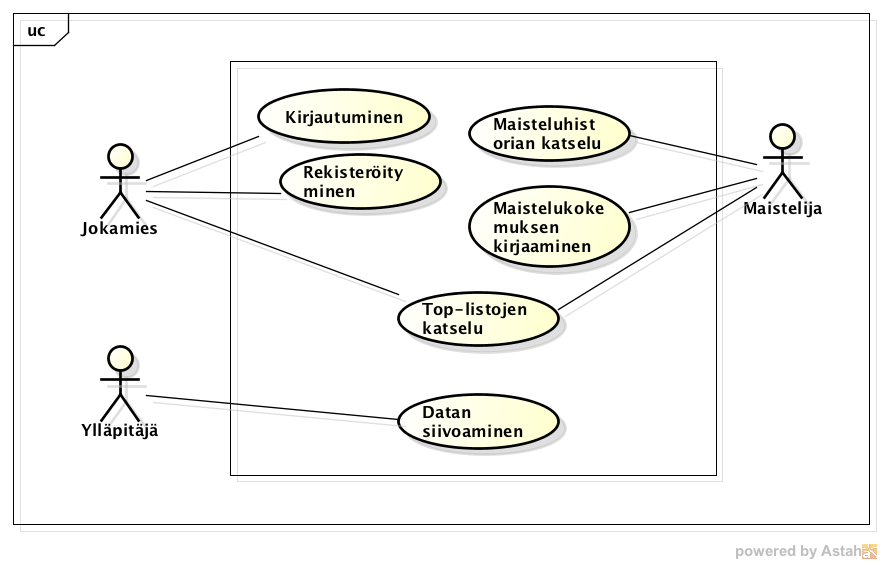
\includegraphics[width=12cm]{usecase}
  \caption{Käyttötapauskaavio}
  \label{fig:käyttötapaus}
\end{figure}

Kuvassa \ref{fig:käyttötapaus} on esitelty sovelluksen käyttäjäryhmät
ja käyttötapaukset. Käyttäjäryhmät ovat:

\begin{description}
\item[Jokamies] Jokamies on kuka tahansa, joka vierailee
  kahvipäiväkirjassa. Kaikki muut käyttäjäryhmät kuuluvat myös tähän
  käyttäjäryhmään.

\item[Maistelija] Maistelija on rekisteröity käyttäjä. Maistelija voi
  lisätä kahvipäiväkirjaan omia maistelukokemuksiaan.

\item[Ylläpitäjä] Ylläpitäjä pitää huolta siitä, että järjestelmään
  syötetty tieto on laadukasta.
\end{description}

\subsection{Jokamiehen käyttötapaukset}

\begin{description}
\item[Top-listojen katselu] Kuka tahansa voi katsella, mitkä kahvit ja
  mitkät kahvilat ovat saaneet parhaat arvosanat sovelluksen
  käyttäjien toimesta.
\end{description}

Muita käyttötapauksia: rekisteröityminen, kirjautuminen.

\subsection{Maistelijan käyttötapaukset}

\begin{description}
\item[Maistelukokemuksen lisääminen] Käyttäjä merkitsee muistiin mitä
  kahvia on juonut, antaa sille arvosanan ja lisää vapaamuotoiset
  muistiinpanot. Jos sovellus ei tunne kahvilaatua entuudestaan, se
  lisätään järjestelmään.

\item[Maisteluhistorian katselu] Käyttäjä pystyy selaamaan
  maistelukokemuksiaan ja saa yhteenvedon maisteluhistoriastaan.
\end{description}

\subsection{Ylläpitäjän käyttötapaukset}

\begin{description}
\item[Datan siivoaminen] Ylläpitäjä voi muokata lisättyjen
  kahvilaatujen tietoja ja tarvittaessa yhdistellä niitä. Esimerkki:
  kaksi käyttäjää ovat lisänneet saman kahvilaadun hieman eri
  nimellä. Ylläpitäjä käy yhdistämässä näiden tiedot.
\end{description}


\section{Järjestelmän tietosisältö}

Järjestelmän tietosisältöä korkealla tasolla kuvaa käsitekaavio
kuvassa \ref{fig:käsitekaavio}.

\begin{figure}[ht]
  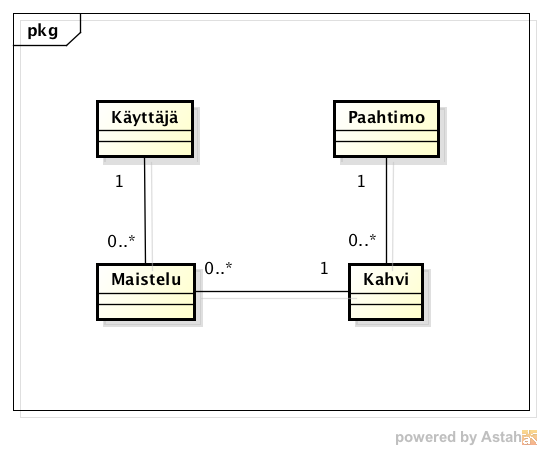
\includegraphics[width=12cm]{database}
  \caption{Käsitekaavio}
  \label{fig:käsitekaavio}
\end{figure}

\subsection{Tietokohde: Käyttäjä}

\begin{center}
\begin{tabularx}{\textwidth}{|X|X|X|}
\hline
Attribuutti & Arvojoukko & Kuvailu \\
\hline
Käyttäjänimi     & Merkkijono & Käyttäjän nimimerkki sovelluksessa. \\
Sähköpostiosoite & Merkkijono & Käyttäjän sähköposti osoite. Mahdollistaa kirjautumisen ja unohtuneen salasanan palauttamisen. \\
Liittymisaika    & Ajanhetki  & Milloin käyttäjätili on luotu. \\
Ylläpitäjyys     & Boolen arvo & Onko käyttäjällä ylläpito-oikeudet. \\
Salasana         & Merkkijono & Salasanan bcrypt-tiiviste. \\
\hline
\end{tabularx}
\end{center}

\subsection{Tietokohde: Paahtimo}

\begin{center}
\begin{tabularx}{\textwidth}{|X|X|X|}
\hline
Attribuutti & Arvojoukko & Kuvailu \\
\hline
Nimi & Merkkijono & Paahtimon nimi. \\
\hline
\end{tabularx}
\end{center}

Kullakin paahtimolla voi olla mielivaltainen määrä kahveja, mutta kukin kahvi voi kuulua vain yhdelle paahtimolle.

\subsection{Tietokohde: Kahvi}

\begin{center}
\begin{tabularx}{\textwidth}{|X|X|X|}
\hline
Attribuutti & Arvojoukko & Kuvailu \\
\hline
Nimi & Merkkijono & Kahvilaadun nimi. \\
\hline
\end{tabularx}
\end{center}

Kukin kahvi kuuluu aina täsmälleen yhdelle paahtimolle.

\subsection{Tietokohde: Maistelu}

\begin{center}
\begin{tabularx}{\textwidth}{ |X|X|X| }
\hline
Attribuutti & Arvojoukko & Kuvailu \\
\hline
Laatu & Merkkijono & Kahvin valmistustapa. \\
Sijainti & Merkkijono & Missä kahvi on nautittu. \\
Arvosana & Kokonaisluku, 1-5 & Yhdestä viiteen tähteä. \\
Muistiinpanot & Merkkijono & Käyttäjän apaamuotoiset muistiinpanot maistelusta. \\
Luontiaika & Ajanhetki & Milloin maistelukokemus on kirjattu. \\
\hline
\end{tabularx}
\end{center}

Kukin maistelukokemus kuuluu käyttäjälle, joka kokemuksen on
kirjannut. Kukin maistelu liittyy aina täsmälleen yhteen kahviin.


\section{Relaatiotietokantakaavio}

Sovelluksen tietokannan rakennetta kuvaa relaatiotietokantakaavio
\ref{fig:relaatiotietokantakaavio}.

\begin{figure}[ht]
  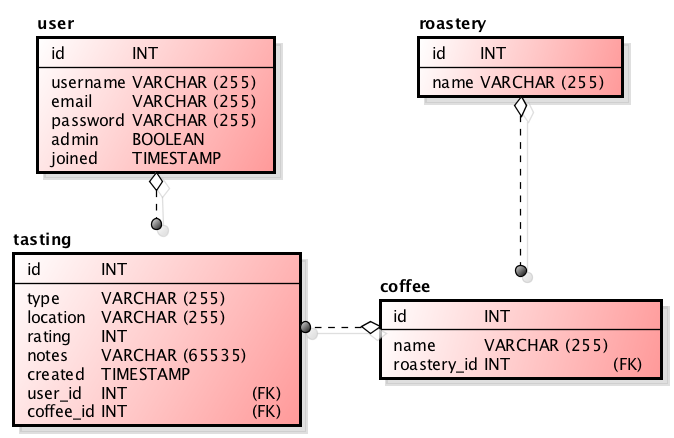
\includegraphics[width=12cm]{relational}
  \caption{Relaatiotietokantakaavio}
  \label{fig:relaatiotietokantakaavio}
\end{figure}


\section{Käyttöliittymä}

Alustava sivukartta on esitetty kuvassa \ref{fig:sivukartta}.

\begin{figure}[ht]
  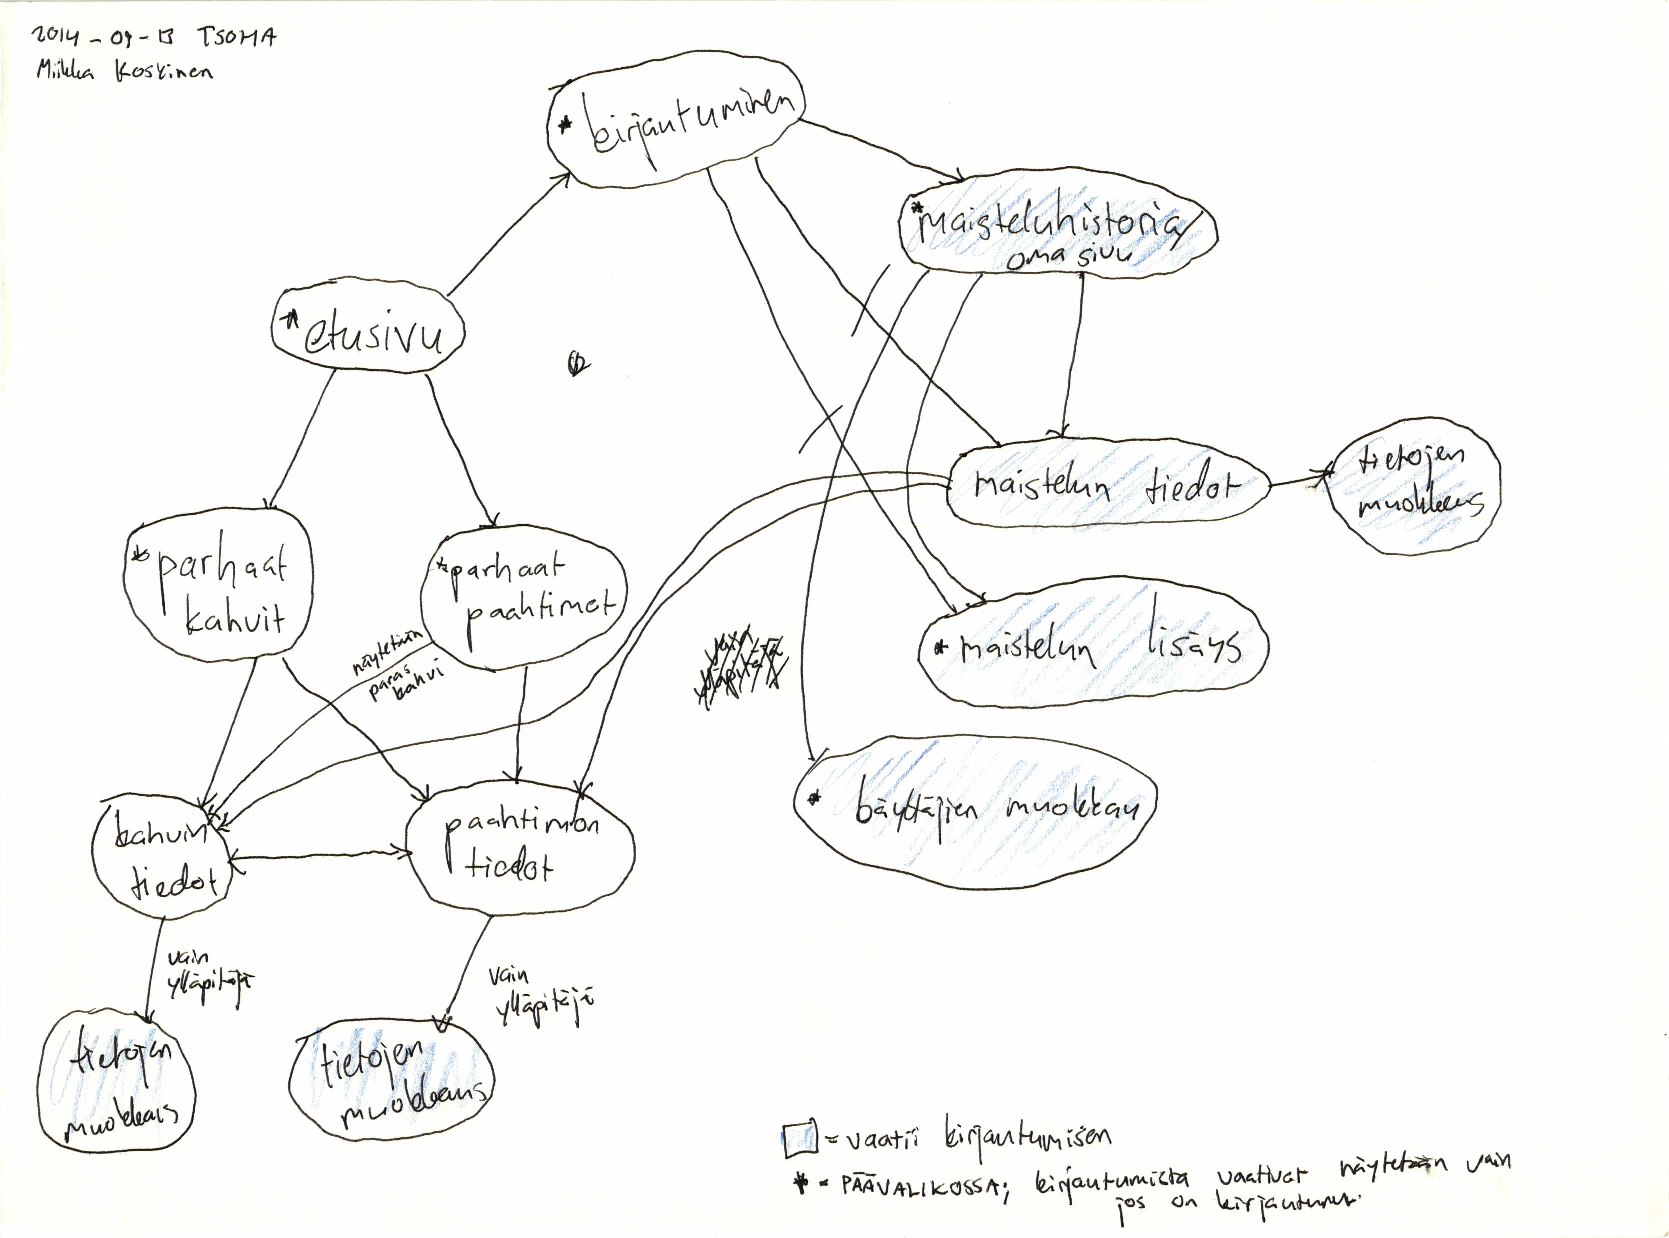
\includegraphics[width=12cm]{ui/sitemap}
  \caption{Alustava sivukartta}
  \label{fig:sivukartta}
\end{figure}



\end{document}
